\subsection{Photometric Calibration}
\label{sec:photometric_calibration}

We have started commissioning the full photometric calibration pipeline for
Rubin Observatory, with great success so far. For testing photometric
calibration we have obtained over 150 dithered science observations in ugriz
over part of the Extended Chandra Deep Field-South (ECDFS) (one of the planned LSST
deep fields), and tens more in rizy over part of the Euclid Deep Field South
(EDFS). All of the science data has delivered seeing of $\sim0.8$ to $\sim1.5$
arcsecond seeing.  The
validation work in this document covers the ECDFS field with its more complete
filter coverage.

The precision photometric calibration software used for Rubin is the Forward
Global Calibration Method (Burke, Rykoff, \etal 2018) which was used
successfully to achieve better than 2 mmag uniformity for the Dark Energy
Survey. This software has been adapted for the LSST Science Pipelines and has
been used on Hyper Suprime Cam Special Survey Program (HSC SSP) for data
releases since DR2.
The performance on HSC data has not been as good as that on DES data due to a
number of reasons, yielding repeatability and uniformity closer to the 5 mmag
level for grizy data.

\iffalse                                % re HSC
First, we have had a lot of problems with HSC
backgrounds and amp-to-amp non-linearities.  Second, the HSC survey strategy
was not well suited to self calibration due to the slow slewing of the
telescope and the long time required to change a filter, leading to lots of
isolated single-band single-night surveys.  Third, we do not have detailed
throughput scans including detector-to-detector QE variations and in-situ scans
of the significant filter variations that are required for the full forward
modeling in FGCM.
\fi

Early calibration of the ComCam data is in many ways easier than that of HSC.
First of all, we have a smaller camera (9 detectors) and thus fewer variations
to have to cross-calibrate.  Second, the camera is situated in the center and
easiest to calibrate part of the focal plane.  Third, we only have one field to
calibrate across a few nights of data so far over a limited range of airmass.
Fourth, the survey strategy (multiple bands per night dithered and repeated
with overlapping filters from night to night) is well suited to
self-calibration.  On the other hand, we do not yet have
detailed filter or detector scans available for ComCam using the CBP (\secRef{cbp}), and are
therefore using the LSSTCam reference filter curves and average detector
throughput for the LSSTCam ITL detectors.  In addition, we do not have a flat
field screen so we have had to rely on twilight flat observations for flat fielding.

\subsubsection{Processing Overview}

We start with the standard ISR as documented in \secRef{isr}. While
there are a number of challenges that we have discovered with the ITL
detectors, these are mostly near the sky level, while the testing of
photometric calibration is focused on brighter stars that are less affected by
these issues. We then apply twilight flats, which we are investigating how to
make better. At the same time, we are going to have the flat field screen and
laser and projector installed prior to the commissioning of LSSTCam, so we do
not want to spend too much time worrying about specific challenges of twilight
flats which are only necessary for ComCam.

After flat fielding we find an initial point-spread function (PSF), do a star
selection based on source and psf moments that was developed for HSC
single-frame processing, and perform an initial astrometric solution and
photometric solution (with a single zero-point per detector).  The initial
astrometric solution is used to associate star observations together prior to
global photometric calibration with FGCM.  The initial photometric solution is
used for rapid analysis and prompt processing, but is not used at all for FGCM
which relies entirely on instrumental fluxes (in units of electrons) with a
minor constraint from the reference catalog.

\subsubsection{Global Photometric Calibration with FGCM}

All associated stars with observations with signal-to-noise greater than 10 are
input into the FGCM solution.  In addition, reference stars from The Monster
reference catalog are associated with the stars.  Only a small fraction of the
reference stars are used in the FGCM solution, sufficient to estimate an
``absolute'' calibration (trusting that The Monster is a good absolute
reference catalog).  There is additional ongoing work with absolute calibration
with respect to the CalSpec star C26202 which is not saturated in LSST images
and is fortunately contained in ECDFS that is described in \secRef{C26202}.

The FGCM model constrains the atmospheric parameters per night, as well as the
absolute throughput relative to the input scans.  The standard atmosphere is
given by MODTRAN, run at the elevation of Cerro Pachon at airmass 1.2 with an
Angstrom aerosol model.  The optics and filters are all taken from
\texttt{lsst/throughputs} version 1.9, and the detector throughput is taken from the
ITL average of the lab scans ingested into \texttt{obs\_lsst\_data}.  Note that the
detector QEs are normalized to 1.0 at 800 nm, which is certainly
greater than the true QE at this wavelength.

\subsubsection{FGCM Results on the ECDFS Field}

The FGCM results presented here are based on the
\texttt{LSSTComCam/runs/DRP/20241101\_20241113/w\_2024\_46/DM-47566} DRP processing
run, specifically the 157 visits overlapping tracts
4847, 4848, 4849, 5062, 5063, 5064 which are in the ECDFS field. Specifically there
are 28, 18, 38, 45, 28 visits in ugriz respectively. All QA plots are available
in \href{https://usdf-rsp.slac.stanford.edu/plot-navigator}{the plot navigator at USDF} in
the collection \texttt{u/erykoff/LSSTComCam/DM-47303/test2/build2/run9}.  In this
section we focus on some of the highlights.

Note that FGCM defines a ``photometric'' observation as one that is consistent
with the forward model, including normal variations in the atmosphere, airmass,
known detector throughputs, filter curves, and additional accomodation for
aperture corrections (discussed in Burke, Rykoff \etal).  With this definition
fully 92\% of the observations were deemed to be photometric by the code.

\subsubsubsection{Illumination Corrections}

Part of the FGCM solution is generating illumination correction maps (\figRef{illumination_correction})
with a second-order 2D Chebyshev polynomial over each detector.  Prior to LSSTCam
commissioning this will be turned into a separate calibration product generated
from dense dithered star field observations (Y1).
We have not yet done dithered observations with ComCam over a dense
field, only high latitude, which limits the precision.  Nevertheless we are
able to constrain reasonable illumination corrections.  The offsets from
detector to detector in the illumination correction are due to unexpected
offsets in the twilight flats that we are investigating.

\begin{figure}
  \begin{center}
    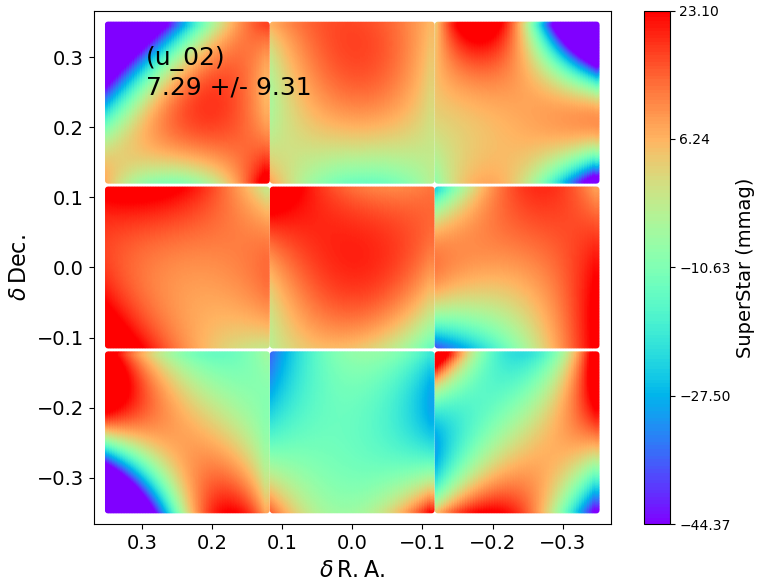
\includegraphics[width=0.3\textwidth]{photometric_calibration_figures/illumcorr_u.png}
    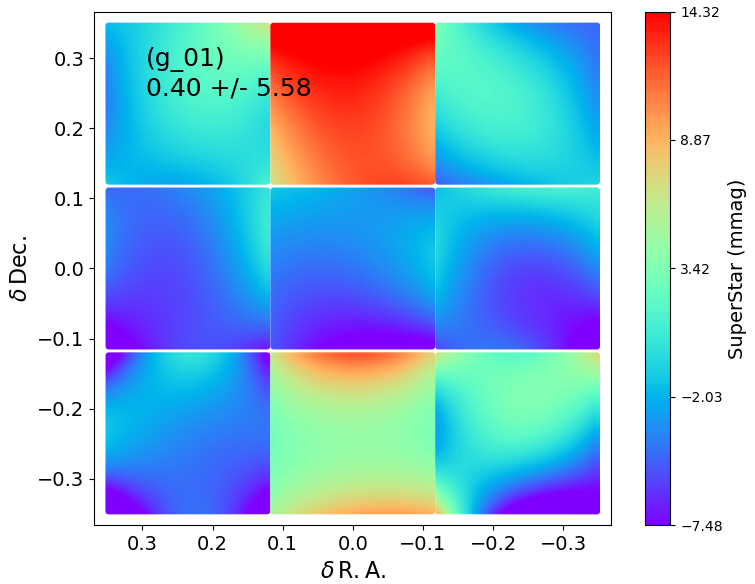
\includegraphics[width=0.3\textwidth]{photometric_calibration_figures/illumcorr_g.png}
    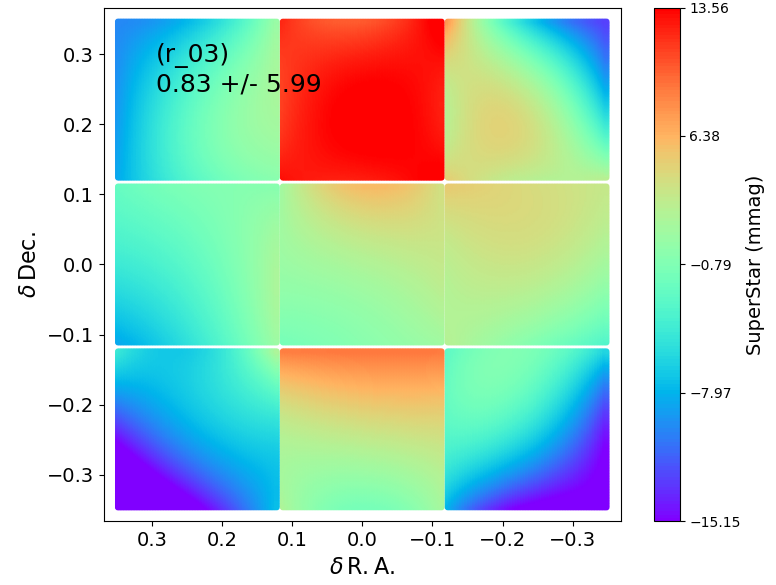
\includegraphics[width=0.3\textwidth]{photometric_calibration_figures/illumcorr_r.png}
    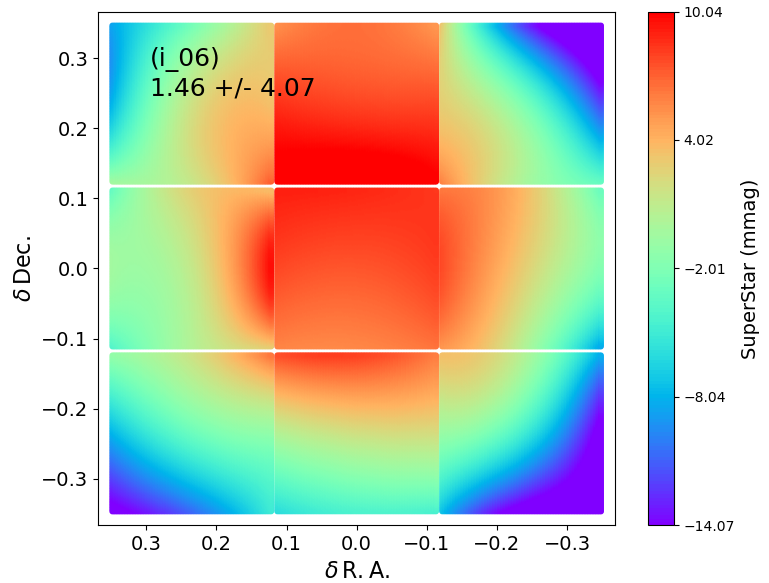
\includegraphics[width=0.3\textwidth]{photometric_calibration_figures/illumcorr_i.png}
    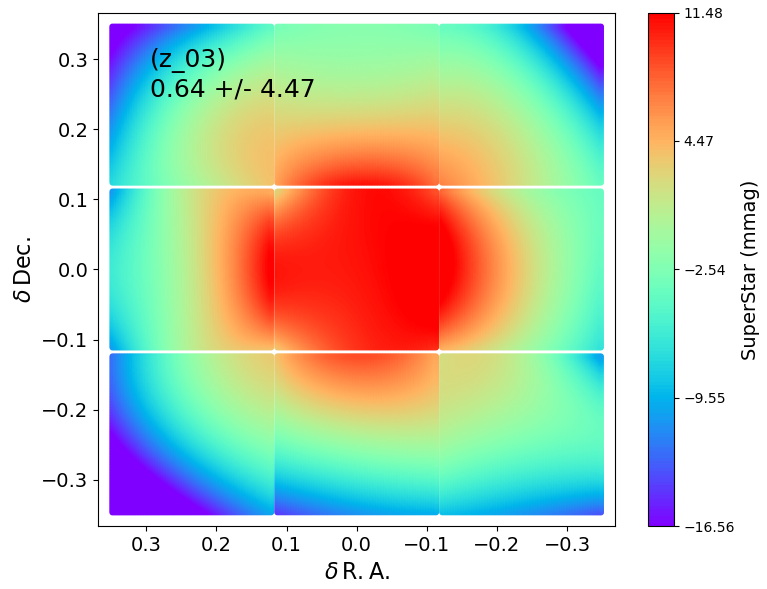
\includegraphics[width=0.3\textwidth]{photometric_calibration_figures/illumcorr_z.png}
  \end{center}
  \caption{Illumination corrections derived from FGCM for the ugriz bands.}
  \label{fig:illumination_correction}
\end{figure}

\subsubsubsection{Photometric Repeatability}

The photometric repeatability after the FGCM fits was excellent. We show here
the repeatability histograms, after all chromatic corrections, for the stars
used in the fit (``all stars'').  Although 10\% of the stars are reserved,
the histograms do not yet have good statistics.  These plots are all made with
signal-to-noise greater than 100 stars (with better than 1\% photometric
errors).  Therefore the scatter is often dominated by photometric error.  The
label ``sigma\_fgcm`` is meant as an estimate of the intrinsic scatter after
subtracting off the photometric error in quadrature. The plots are split into
four panels, showing all stars, the 25\% bluest (from $g-i$ color), the 50\%
middle color, and the 25\% reddest stars. Note that the reddest stars tend to
be fainter and thus have larger photometric error. Furthermore, there are no
red stars observed in the u-band. In all cases except the u-band the intrinsic
repeatability is $1\,\mathrm{mmag}$ or better, and for the u-band it is better
than $5\,\mathrm{mmag}$, comfortably exceeding our requirements in all measured bands.

\begin{figure}
  \begin{center}
    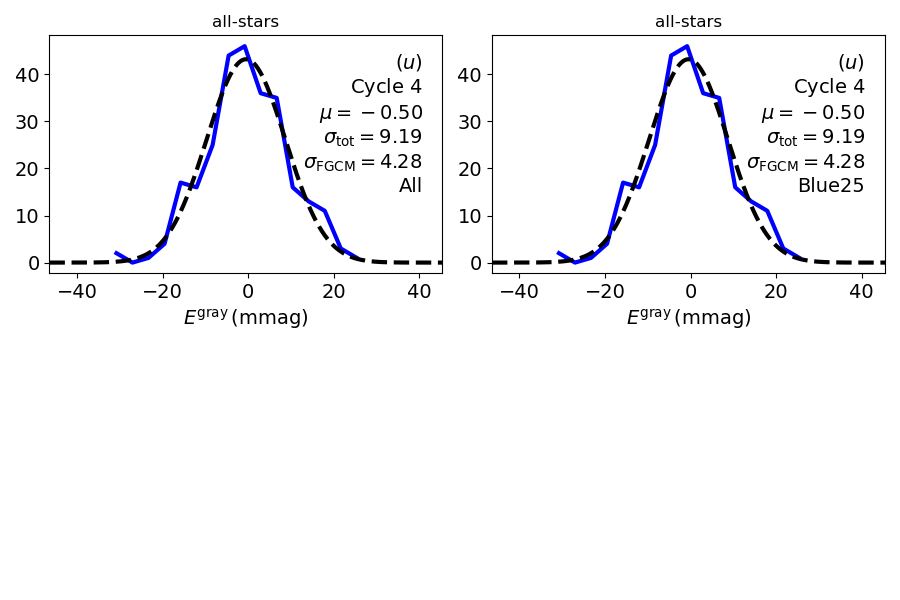
\includegraphics[width=0.3\textwidth]{photometric_calibration_figures/repeatability_u.png}
    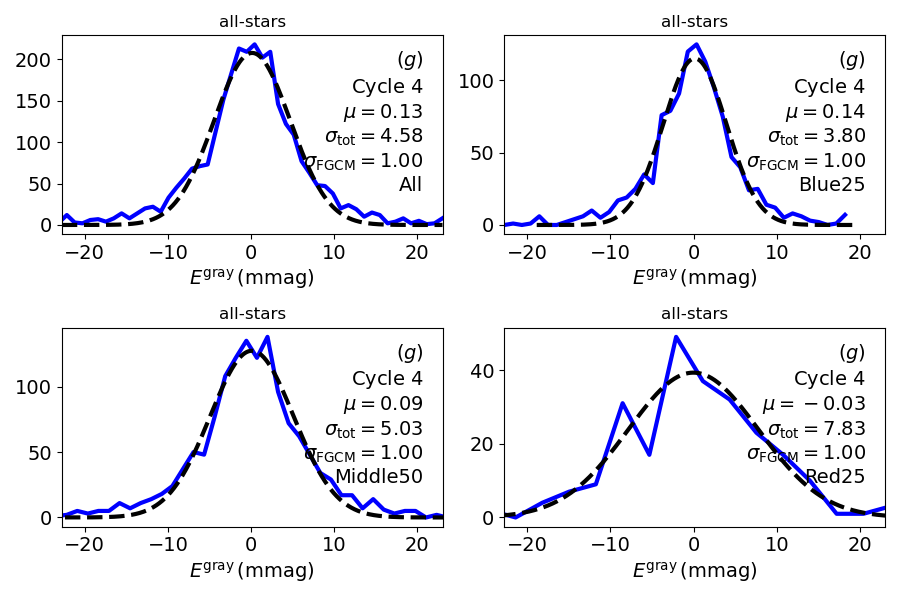
\includegraphics[width=0.3\textwidth]{photometric_calibration_figures/repeatability_g.png}
    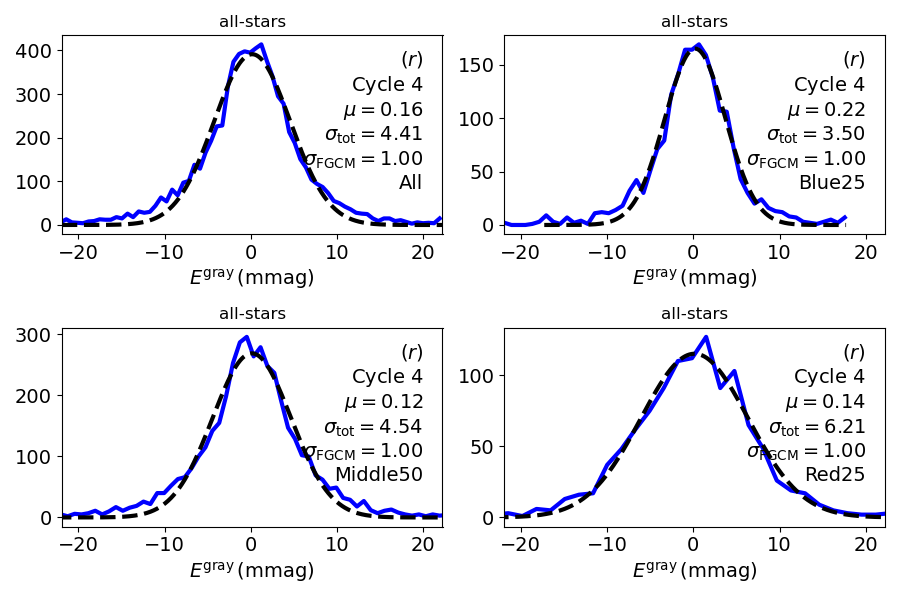
\includegraphics[width=0.3\textwidth]{photometric_calibration_figures/repeatability_r.png}
    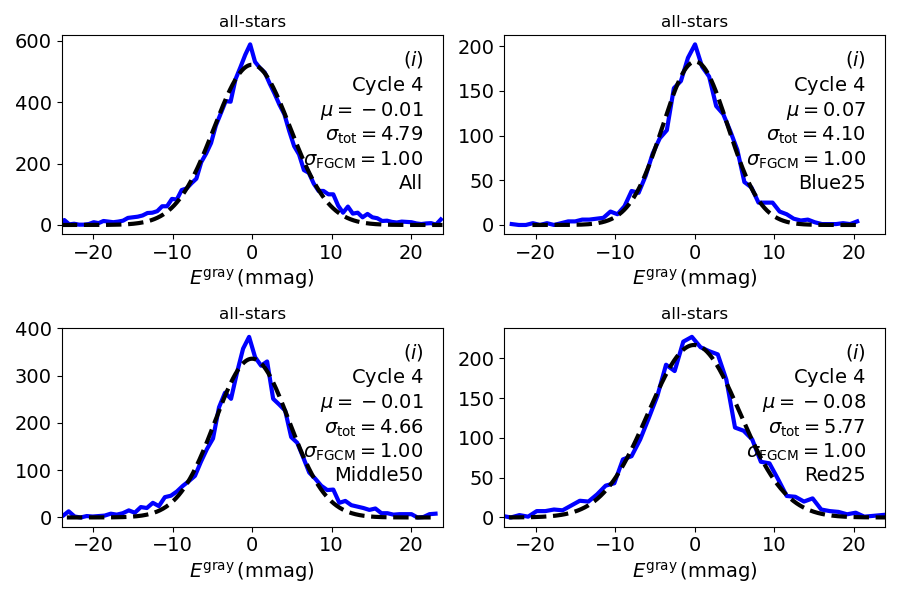
\includegraphics[width=0.3\textwidth]{photometric_calibration_figures/repeatability_i.png}
    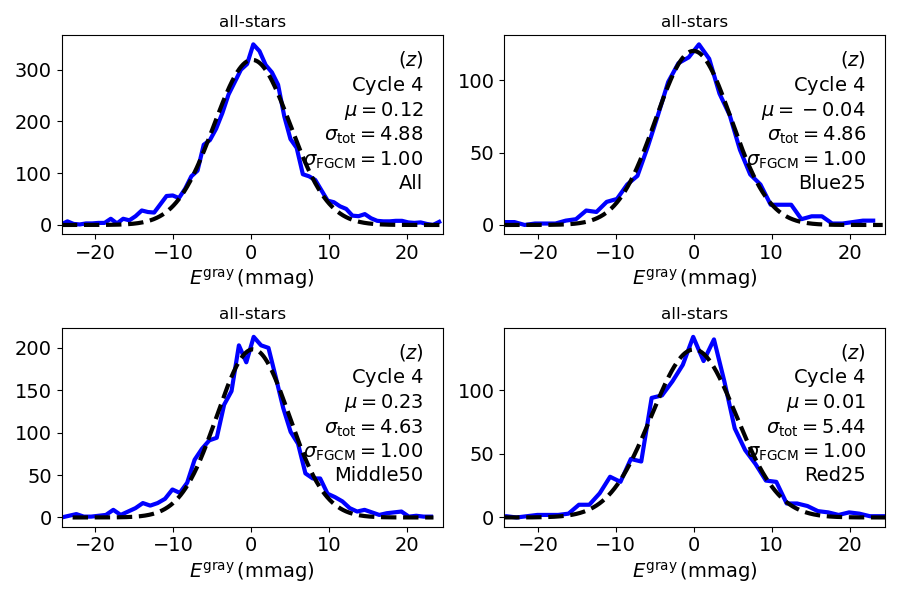
\includegraphics[width=0.3\textwidth]{photometric_calibration_figures/repeatability_z.png}
  \end{center}
  \caption{Photometric repeatability for stars in the ugriz bands.}
\end{figure}

\subsubsubsection{Detector Chromaticity Fits}

In the absence of full in-situ throughput scans, we additionally constrain the
``chromaticity'' of the detectors, which is a first-order adjustment to the
slope of the peak of the throughput curve per-detector.  By doing this
adjustment in throughput space rather than color space we can preserve the
forward model approach, and additionally apply these corrections to any
SED. Note that this operation assumes that the filters are perfectly known, and
it is only the detector throughput that is varying.  This is, in general, a
valid assumption in the g band where the AR coating varies from detector to
detector causing chromatic differences in this band.

\begin{figure}
  \begin{center}
    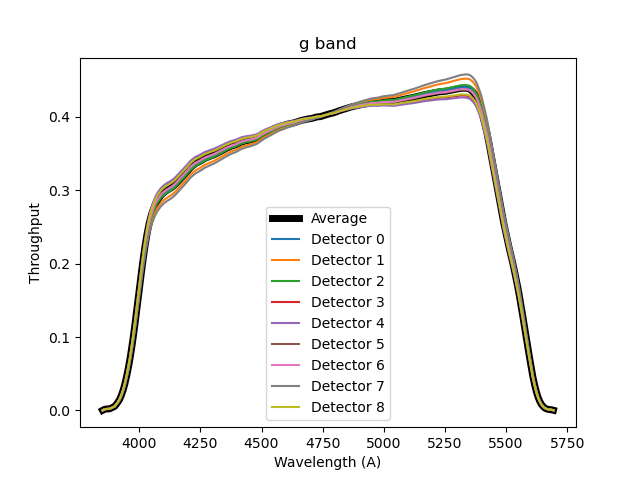
\includegraphics[width=0.6\textwidth]{photometric_calibration_figures/detector_chromaticity_g.png}
  \end{center}
  \caption{Variation in throughput in the g band for the 9 ComCam detectors as
    derived from star colors. These are all constrained relative to the average
    ITL throughput. The CBP will be used for making this measurement
    ``correctly'', but this serves as a prediction of what variations the CBP
    scans should observe when we have it running on ComCam.}
\end{figure}

\subsubsubsection{Absolute Throughputs}
\label{sec:absolutethroughputs}

The FGCM fit performs a ``dead reckoning'' of the expected absolute throughput
given the telescope aperture, the effective gain, the standard atmosphere, and
the various throughputs input.  See above for the throughputs assumed.  If we
trust The Monster reference catalog for absolute calibration,
\figRef{absthroughputs} shows the comparison of the delivered
throughput to the predicted throughput.  In griz bands it is very close, given
that (a) we know that the peak detector QE is not 100\%; and (b) the ComCam
front lens did not have an AR coat applied, thus reducing its throughput
relative to nominal LSSTCam lenses.  In u band we are getting more throughput
than predicted.  This may be an issue with the reference catalog, or our ComCam
u-band QE is 20-30\% larger than the baseline expectation.  Given how fast the
detector QE falls off in the u-band, it would not take much to increase the
throughput by this factor.

\begin{figure}
  \begin{center}
    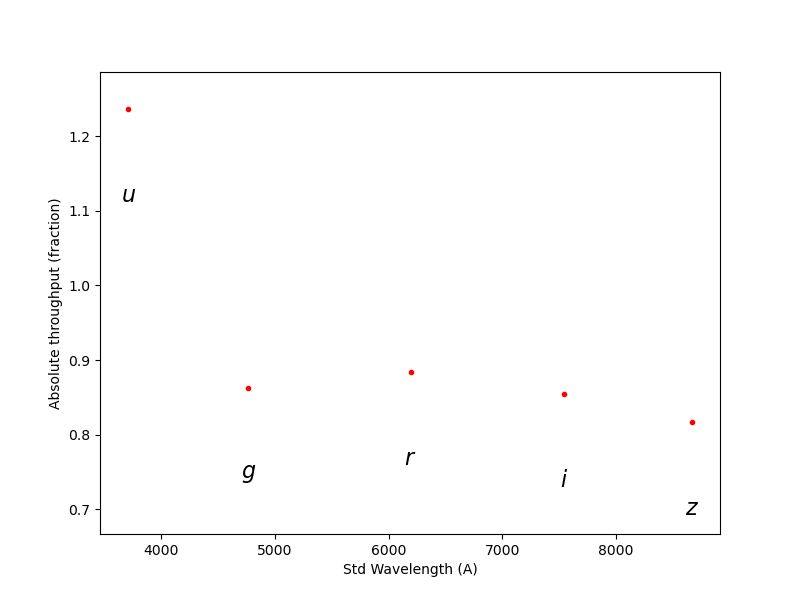
\includegraphics[width=0.6\textwidth]{photometric_calibration_figures/abs_throughput.png}
  \end{center}
  \caption{Absolute throughput derived per band, relative to naive expectations.}
  \label{fig:absthroughputs}
\end{figure}

We have additional ongoing studies of absolute throughputs using the CalSpec
standard C26202 directly.

\subsubsubsection{Comparison to The Monster}

Given our calibrated stars from the FGCM fit we can compare the magnitudes as a
function of color against The Monster reference catalog.  The ``lsst'' fluxes
in The Monster were derived by using stellar spectra to convert from The
Monster native DES system to the standard throughputs in lsst/throughputs
v1.9. These do not match ComCam, in particular it used a strange hybrid of
ITL/E2V for the detector throughput, which is not correct for
ComCam. Therefore, we do expect residual color terms.  Studies are ongoing on
whether these color terms are expected given the differences between the ComCam
throughput and the predicted LSST throughput.  Further validation will be
possible if we get CBP scans prior to the removal of ComCam.

\begin{figure}
  \begin{center}
    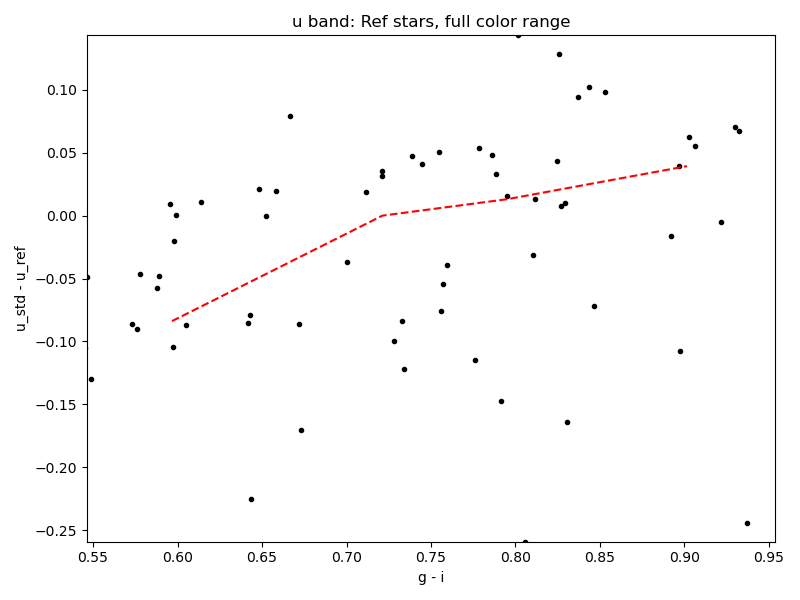
\includegraphics[width=0.3\textwidth]{photometric_calibration_figures/reference_residuals_u.png}
    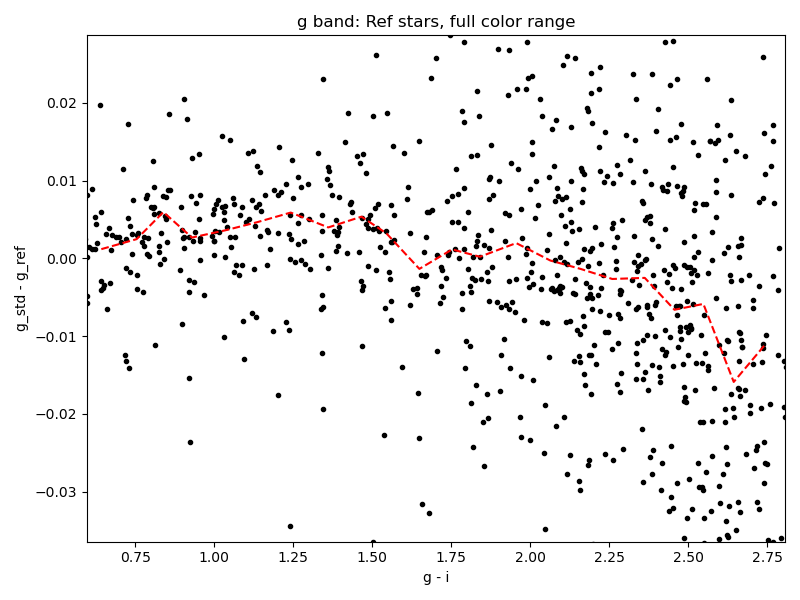
\includegraphics[width=0.3\textwidth]{photometric_calibration_figures/reference_residuals_g.png}
    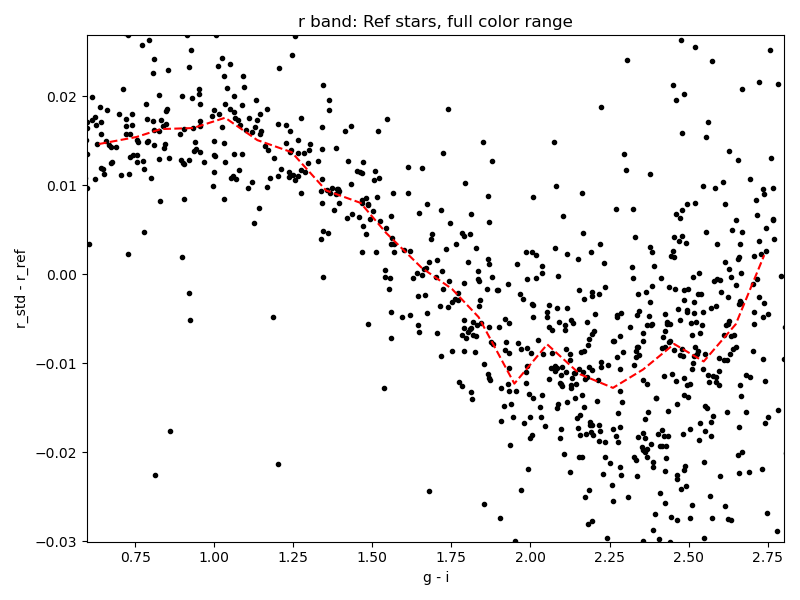
\includegraphics[width=0.3\textwidth]{photometric_calibration_figures/reference_residuals_r.png}
    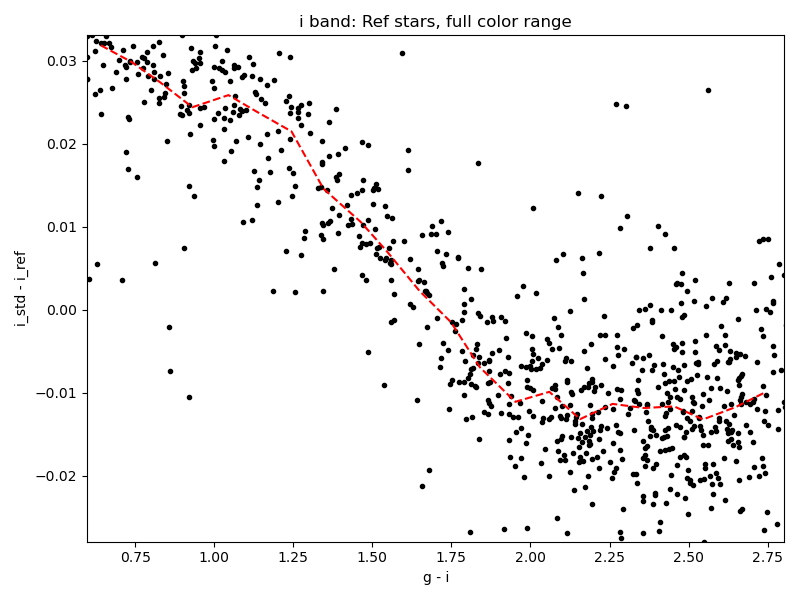
\includegraphics[width=0.3\textwidth]{photometric_calibration_figures/reference_residuals_i.png}
    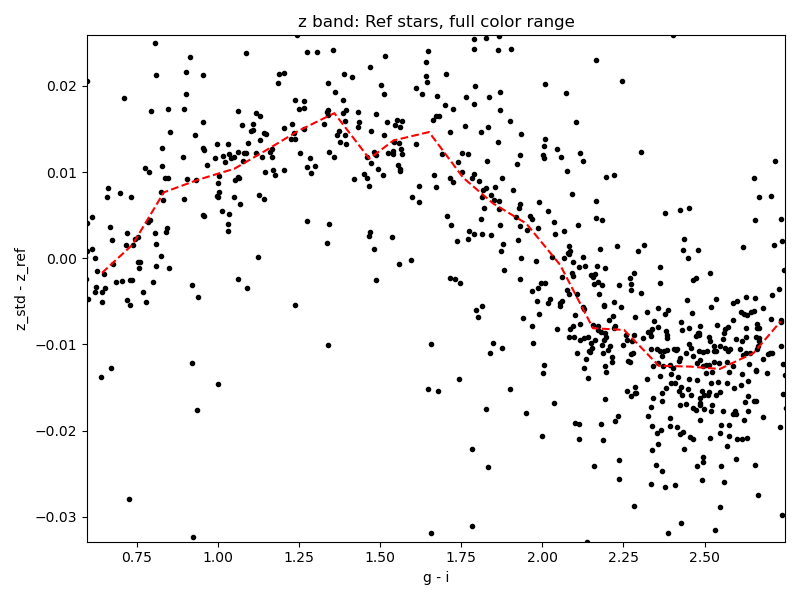
\includegraphics[width=0.3\textwidth]{photometric_calibration_figures/reference_residuals_z.png}
  \end{center}
  \caption{Residuals between FGCM standardized magnitudes and The Monster
    predicted LSST magnitudes for the ugriz bands as a function of $g-i$, assuming
    The Monster has the correct absolute throughput.}
\end{figure}

\subsubsubsection{Background Oversubtraction}

As a side-effect in the calibration, FGCM tests local background
oversubtraction by looking at the statistical difference between two large
aperture magnitudes.  If the background were perfectly measured then the
difference in magnitude will just be a measure of the wings of the PSF (a local
portion of the growth curve) which should be self-similar for all star fluxes.
Instead, we generally see a downturn consistent with a constant background
offset.  This background oversubtraction has been seen in DES, HSC, and
ComCamSim data at similar levels with different photometric pipelines.  It is
worse in the redder bands.  It seems to be caused by the far wings of stars (in
DES all stars and galaxies brighter than 17th magnitude in i contribute), as
well as possibly due to faint undetected sources.  This same background
oversubtraction effect is seen in the ComCam images.  Further investigations
are being done by the low-surface-brightness science unit.

\begin{figure}
  \begin{center}
    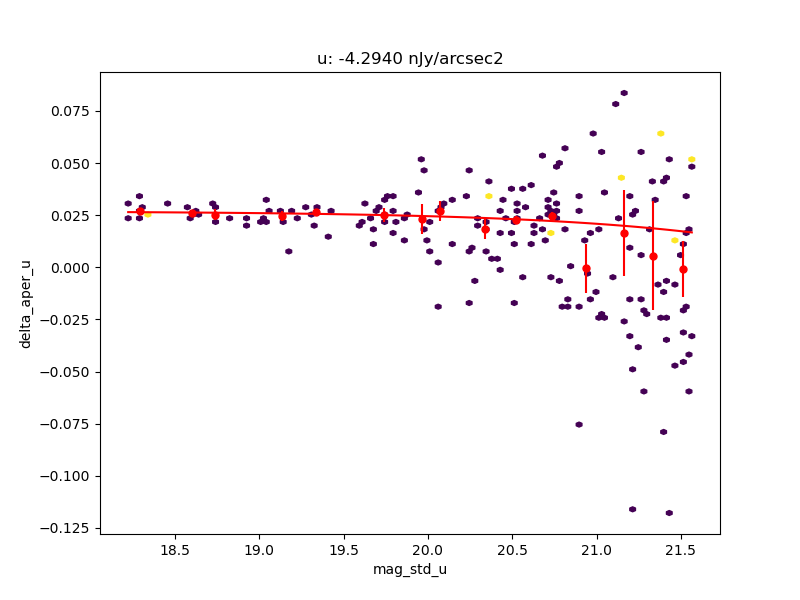
\includegraphics[width=0.3\textwidth]{photometric_calibration_figures/background_oversubtraction_u.png}
    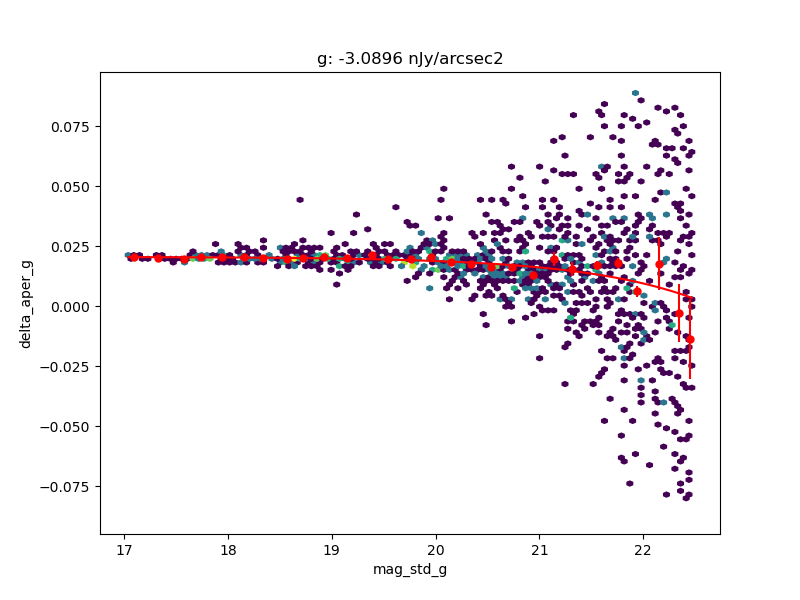
\includegraphics[width=0.3\textwidth]{photometric_calibration_figures/background_oversubtraction_g.png}
    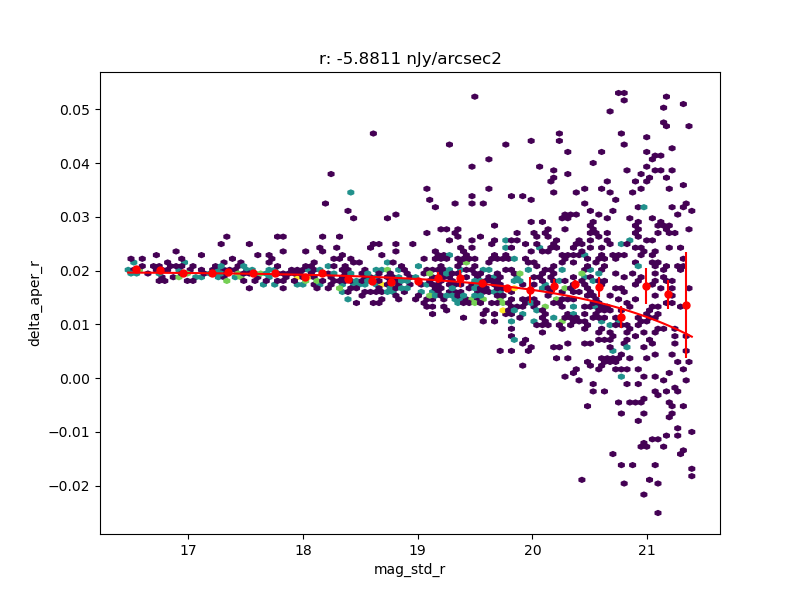
\includegraphics[width=0.3\textwidth]{photometric_calibration_figures/background_oversubtraction_r.png}
    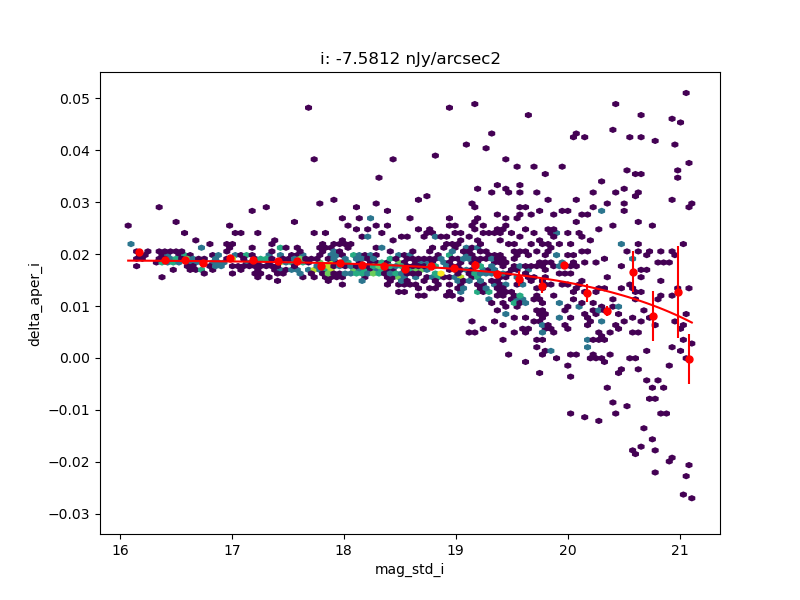
\includegraphics[width=0.3\textwidth]{photometric_calibration_figures/background_oversubtraction_i.png}
    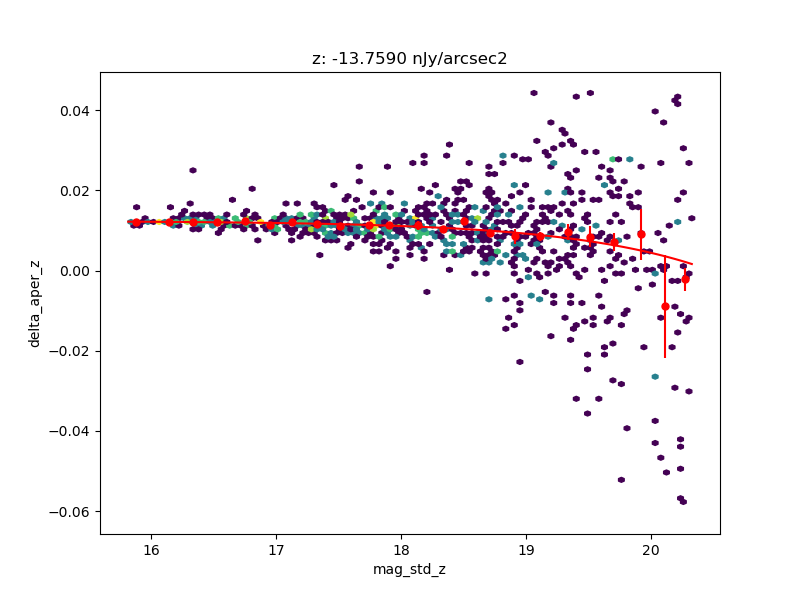
\includegraphics[width=0.3\textwidth]{photometric_calibration_figures/background_oversubtraction_z.png}
  \end{center}
  \caption{Estimate of the background oversubtraction using delta magnitudes
    from large apertures in the ugriz bands.  The amount of curvature is a measure
    of the oversubtraction; this should be flat as a function of star magnitude
    if the background were measured correctly on average.}
\end{figure}

\begin{figure}
  \begin{center}
    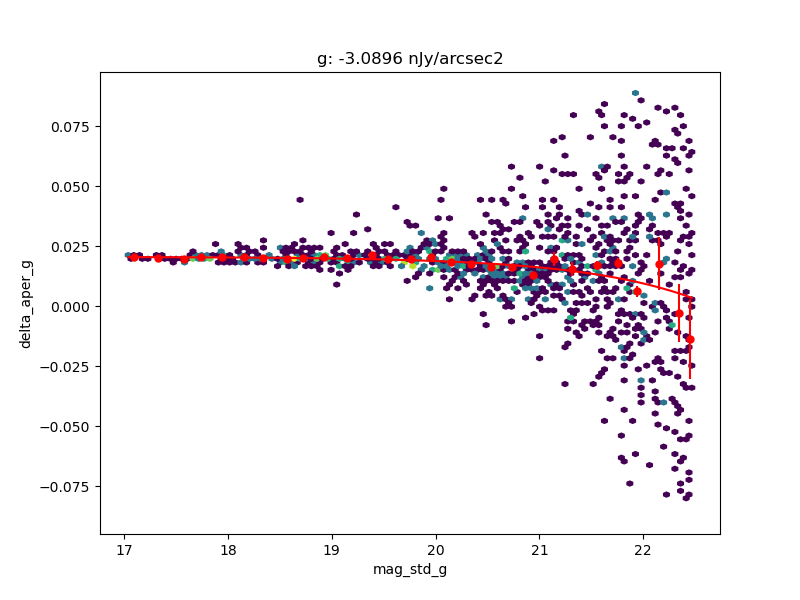
\includegraphics[width=0.45\textwidth]{photometric_calibration_figures/background_oversubtraction_g.png}
    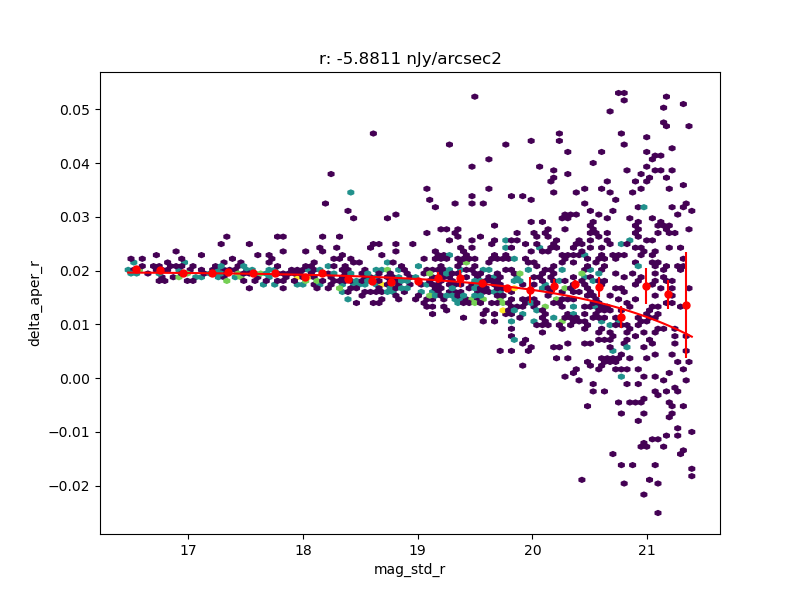
\includegraphics[width=0.45\textwidth]{photometric_calibration_figures/background_oversubtraction_r.png}
    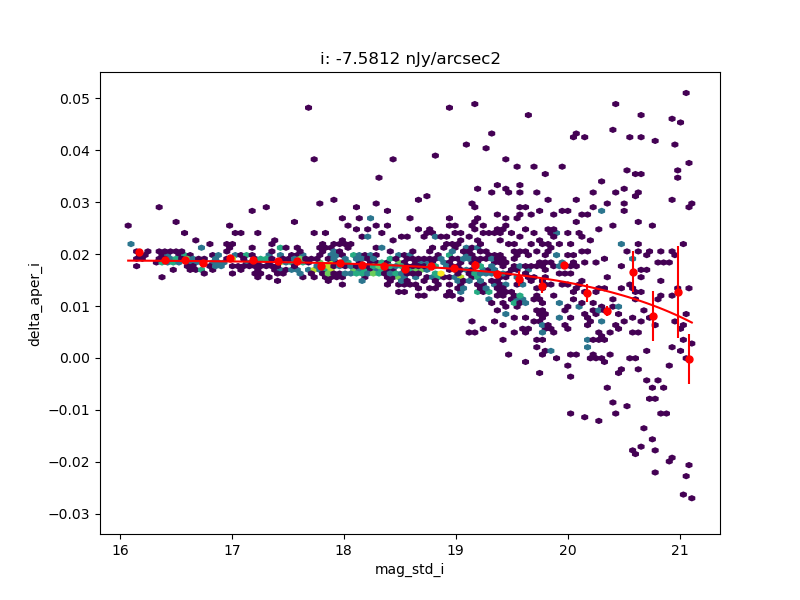
\includegraphics[width=0.45\textwidth]{photometric_calibration_figures/background_oversubtraction_i.png}
    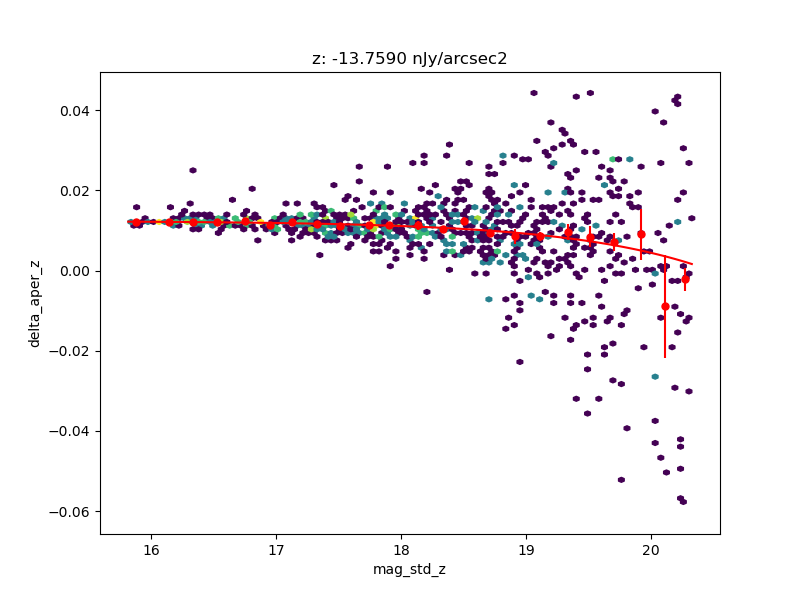
\includegraphics[width=0.45\textwidth]{photometric_calibration_figures/background_oversubtraction_z.png}
  \end{center}
  \caption{Estimate of the background oversubtraction using delta magnitudes
    from large apertures in the griz bands.  The amount of curvature is a measure
    of the oversubtraction; this should be flat as a function of star magnitude
    if the background were measured correctly on average.}
\end{figure}

\subsubsection{Next Steps}

The following additional data will need be taken to advance from our current
knowledge:

\begin{enumerate}
  \item{g band observations in the EDFS field, when the g filter is put back
    into ComCam for the upcoming dark time.}
  \item{Dithered observations in as many bands as possible over a field with
    much larger stellar density for better illumination corrections.}
  \item{More contiguous dithered survey data in (at least) gri.}
\end{enumerate}

The particular emphasis on g band in these requests is that by default FGCM
will use the $g-i$ color for internal QA, which is a very useful color to split
on.  There are no facilities in the code for doing quality calibrations on
multiple disconnected fields with different band coverage, as this is not the
normal case for survey observations.  We could run different fields separately
with different configs, but this is not preferred.  Thus, gri coverage over the
fields of interest for DRP processing is the ``easiest'' path that will yield
the best results and be most consistent with the LSST survey.


\subsection{A Comparison with the HST CalSpec Standard C26202}
\label{sec:C26202}

The CDFS field observed by ComCam during commissioning contains an HST
CalSpec standard that is faint enough not to saturate the ComCam
science images.  This HST CalSpec
standard\footnote{\url{https://www.stsci.edu/hst/instrumentation/reference-data-for-calibration-and-tools/astronomical-catalogs/calspec}},
C26202, had previously been used to perform the absolute AB
calibration of the Dark Energy Survey (DES) Data Release 2 (DR2)
\citep{2021ApJS..255...20A}.

For the ComCam data, two separate (but related) analyses were
performed using the ComCam observations of C26202: (1) a measurement
of the absolute system throughput of the ComCam $ugrizy$ bandpasses,
and (2) a measurement of how far off the initial absolute photometric
calibrations were from the AB magnitude system (``AB offsets'') for
these same bandpasses.

These two analyses are discussed below.

\subsubsection{Absolute System Throughput Measurements}

For the absolute system throughput analysis, the expected total counts
(in electrons) for C26202 were calculated for each of the ComCam
bandpasses for a 30-second exposure, assuming the engineering system
throughputs for an average ITL CCD found in the {\tt
  syseng\_throughputs repository} (see
\url{https://github.com/lsst-pst/syseng\_throughputs}). Expected
counts in each filter passband were calculated for a range of
airmasses ($1.0 \leq X \leq 2.5$) in steps of 0.1 airmass to cover the
full range of possible airmasses of the observed ComCam data.
Throughout, the HST CalSpec spectral energy distribution (SED), {\tt
  c26202\_stiswfcnic\_007.fits}, was used as the C26202
spectrophotometric reference spectrum.

Next, the post-ISR instrumental counts (in electrons) for C26202 were
retrieved from the {\tt icSrc} tables from the ComCam observations in
the Butler at the USDF.  The {\tt base\_PsfFlux\_instFlux} was used,
and an aperture correction from PSF to total flux was applied making
use of the {\tt base\_CircularApertureFlux\_70} as a proxy for total
instrumental flux.

Finally, for each of the $ugrizy$ filter passbands, the ratio of the
observed total flux to the expected (synthetic) total flux was
calculated and plotted.  The results can be found in
Figure~\ref{fig:c26202_throughputs}.  Note that the measured and
predicted counts from per-visit synthetic photometry is consistent for
all bands at the $\sim$5\% level.

\begin{figure}
  \begin{center}
    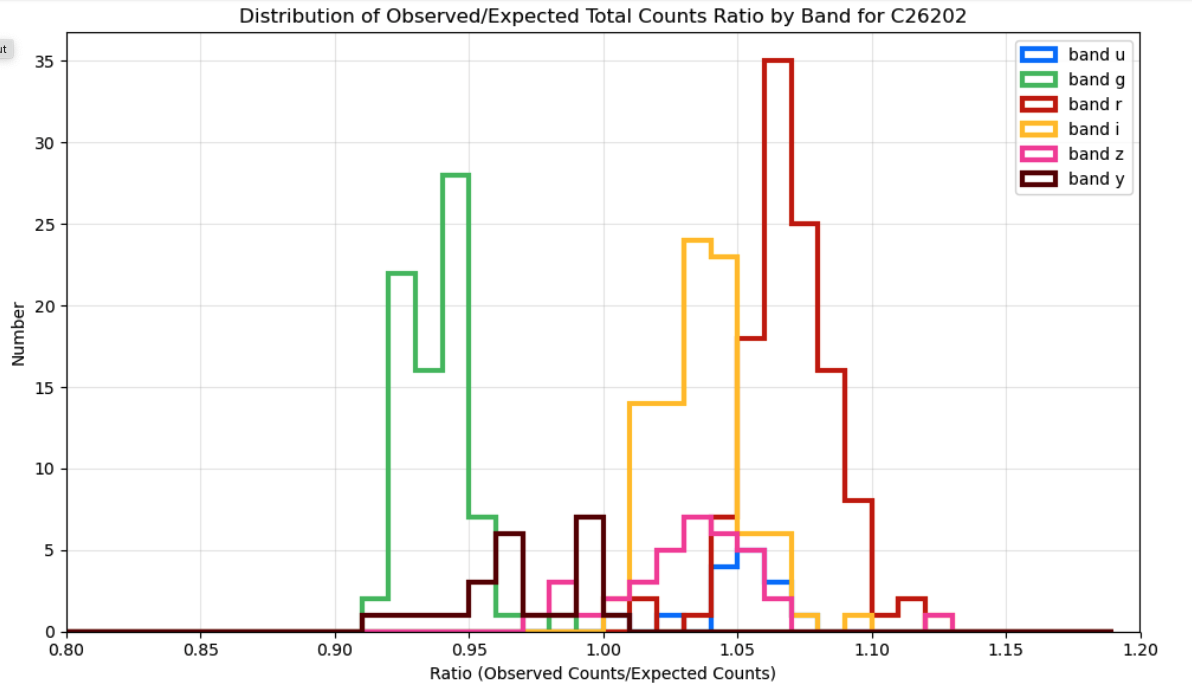
\includegraphics[width=0.7\textwidth]{photometric_calibration_figures/LSSTComCam_Absolute_Throughputs_20241210.png}
  \end{center}
  \caption{\label{fig:c26202_throughputs}The histogram of the ratio of
    the observed counts to the expected counts for HST CalSpec
    spectrophotometric standard star C26202 from ComCam observations
    in {\tt
      LSSTComCam/runs/DRP/20241101\_20241204/w\_2024\_49/DM-47988}.
    Median values of the ratio for each passband are: 1.053 ($u$),
    0.939 ($g$), 1.068 ($r$), 1.037 ($i$), 1.037 ($z$), and 0.967
    ($y$).}
  \label{fig:c26202_ab_offsets}
\end{figure}


\subsubsection{AB Offsets}

The C26202 AB magnitude offsets are the difference between the
calibrated observed ComCam AB magnitudes and the {\tt
  rubin\_sim.PhotUtils}-determined synthetic AB magnitudes for the
ComCam $ugrizy$ filter passbands.

The calibrated ComCam AB magnitudes in each of the passbands are
obtained by converting the {\tt calibFlux} values in the USDF butler
{\tt sourceTable} from nano-Janskys to AB magnitudes via the equation
$mag_{\rm ab} = -2.5 \times log_{10}(calibFlux) + 31.4$.

As with the absolute system throughput measurements for the expected
counts of C26202, the engineering system throughputs for an average
ITL CCD found in the {\tt syseng\_throughputs repository} were used
for calculating the expected AB magnitudes with the {\tt rubin\_sim
  PhotUtils} module for each filter bandpass.  Also, as with the
absolute system throughput measurements, the HST CalSpec spectral
energy distribution (SED), {\tt c26202\_stiswfcnic\_007.fits}, was
used as the C26202 spectrophotometric reference spectrum.

The results are shown in \ref{tab:C26202}.

These results are not unexpected, as performing absolute calibrations
on reference catalog data is extremely difficult before real observed
data are obtained in a new filter bandpass system.  Updates are now
being applied by the Rubin Calibration Scientist to address these
offsets.


\begin{table*}
\centering
\begin{tabular}{@{}lcccc@{}}
  Band & No. of \ComCam observations & median \ComCam mag. & CalSpec synthetic mag. & offset \\
  \hline
u             & 28  & 17.869 & 17.573 &  $\phantom{-}0.296$ \\
g             & 77  & 16.684 & 16.692 &  $          -0.008$ \\
r             & 121 & 16.269 & 16.362 &  $          -0.093$ \\
i             & 99  & 16.197 & 16.260 &  $          -0.063$ \\
z             & 42  & 16.589 & 16.244 &  $\phantom{-}0.346$ \\
y             & 24  & 16.269 & 16.239 &  $\phantom{-}0.031$ \\
\end{tabular}
\caption{Comparison of \ComCam observed magnitudes with synthetic magnitudes calculated from
  C26202\_stiswfcnic\_007 using \ComCam passbands.
}
\label{tab:C26202}
\end{table*}

%HST CalSpec Standard observed in ECDFS field

%DRP Cumulative collection \texttt{LSSTComCam/runs/DRP/20241101_20241204/w_2024_49/DM-47988}
%ComCam observed mags are from the calibFlux values from the sourceTable

%ComCam ugrizy synthetic mags generated using rubin_sim.PhotUtils and syseng_throughput
%ComCam ITL responses used.

%There are 2 related-but-separate analyses going on:  the AB offset analysis here, and 
%the throughput analysis.
%The AB offset analysis is just concerned about the difference in the calibrated observed 
%ConCam AB magnitudes and the synthetic AB magnitudes.  We get the calibrated ConCom AB 
%magnitudes from the calibFlux column of the sourceTable and converting the calibFlux 
%(in nano-Janskys) to AB magnitudess via mag_ab = -2.5*log10(calibFlux).   I believe — 
% but am not 100% certain — that the calibFlux values in the sourceTable have been 
%photometrically calibrated against the Monster RefCat, probably via calculating a local 
%photometric zeropoint from the Monster stars observed by ConCam in that visit+detector.  
%If this is the procedure for the photometric calibration of the calibFlux column of the 
%sourceTable, the first-order airmass correction (the k*X term in SDSS parlance) is taken 
%care of automatically, since the Monster RefCat stars are observed through the same airmass 
%for that  visit+detector.  For the synthetic AB magnitudes, essentially Equation 7 of 
%Fukugita \etal (1996) is used.  The shape of the passbands is important, but the total 
%throughput cancels out.  For the ConCam-based synthetic magnitudes, I used the rubin_sim 
%PhotUtils module and the syseng_throughput package (in order to make use of the ConCam 
%ITL responses), following code that Lynne Jones pointed me to.  (I think the default 
%airmass is X=1.2 or X=1.3; I am not sure, but it shouldn’t make a bit difference in the 
%overall shape of the passbands.) So, if the passband shapes (including atmosphere, etc.) 
%are generally well known and if the calibFlux is indeed calibrated against the Monster 
%RefCat,  but there is an overall AB magnitude offset, I think this would imply a possible 
%AB calibration error in the Monster RefCat.

%The total throughput analysis ignores the Monster entirely.  It takes the ISR-corrected 
%(but not photometrically zeropointed) psf instFlux counts for C26202 from the icSrc 
%table and compares them against the expected counts for a single 30-second exposure 
%calculated via rubin_sim PhotUtils module and the syseng_throughput package, again 
%making use of code that Lynne provided.  In this case, estimaging total throughput 
%is critical to the analysis — in fact, it is the purpose of the analysis.   Here, 
%the expected counts are corrected to the airmass of the visit, and not just to a 
%typical/official airmass like in the AB offset analysis above.
